\documentclass[conference]{IEEEtran}
\IEEEoverridecommandlockouts

% Packages
\usepackage{cite}
\usepackage{amsmath,amsfonts,amssymb}
\usepackage{graphicx}
\usepackage{multirow}
\usepackage{booktabs}
\usepackage{siunitx}
\usepackage{algorithm}
\usepackage{algpseudocode}
\usepackage{mathtools}
\usepackage{array}
\usepackage{xcolor}
\usepackage{subcaption}
\usepackage{url}
\usepackage{hyperref}
\usepackage{float}

\begin{document}

\title{Privacy-Preserving Health Data Exchange Using Secure Multi-Party Computation}

\title{Privacy-Preserving Health Data Exchange Using Secure Multi-Party Computation}

\author{
\IEEEauthorblockN{Lokesh Chowdary K}
\IEEEauthorblockA{
Dept of CSE - Cyber Security \\
RNS Institute of Technology \\
Bengaluru, India \\
%Email: lokesh.chowdary.k@rnsit.edu.in
}
\and
\IEEEauthorblockN{Shashank L}
\IEEEauthorblockA{
Dept of CSE - Cyber Security \\
RNS Institute of Technology \\
Bengaluru, India \\
%Email: shashank.l@rnsit.edu.in
}
\and
\IEEEauthorblockN{Mrs. Latha P}
\IEEEauthorblockA{
Asst. Prof, Dept of CSE - Cyber Security \\
RNS Institute of Technology \\
Bengaluru, India \\
%Email: lathap@rnsit.edu.in
}
}

\maketitle

\begin{abstract}
The need for collaborative data analytics in healthcare is rapidly increasing, yet stringent privacy regulations and ethical concerns often prevent institutions from sharing sensitive patient data. Traditional anonymization techniques are insufficient against modern re-identification risks, highlighting the need for cryptographic approaches that enable analysis without revealing raw data. In this paper, we present a comprehensive platform for privacy-preserving health data exchange based on Secure Multi-Party Computation (SMPC), opportunistic Homomorphic Encryption (HE), and optional Differential Privacy (DP). The system supports eighteen categories of statistical and machine learning analytics, from descriptive statistics and correlation to regression, survival analysis, and federated learning. It integrates a full-stack architecture with secure computation, orchestration, monitoring, and compliance components. Experimental results show that our secure computations achieve near-identical accuracy to plaintext baselines and scale linearly with dataset size. We further provide deployment guidelines, security analysis, and a real-world case study to illustrate the platform's practicality. This work demonstrates that privacy-preserving healthcare analytics is not only theoretically feasible but also deployable in real clinical settings.
\end{abstract}

\begin{IEEEkeywords}
Secure Multi-Party Computation, Homomorphic Encryption, Healthcare Analytics, Data Privacy, Differential Privacy, Federated Learning
\end{IEEEkeywords}

\section{Introduction}
Healthcare institutions increasingly rely on data analytics to improve diagnosis, treatment planning, resource allocation, and epidemiological modeling. The quality and diversity of data play a crucial role in improving predictive models and clinical decision-making. However, stringent privacy laws such as HIPAA in the United States and GDPR in the European Union impose strict restrictions on sharing identifiable patient information. These legal and ethical constraints create a significant tension between the need for collaborative analytics and the obligation to protect sensitive data.

Traditional methods such as anonymization and de-identification offer limited protection, as numerous studies have demonstrated the ease of re-identification through auxiliary datasets. As a result, cryptographic approaches that enable joint computation without data exposure are emerging as a preferred alternative. Secure Multi-Party Computation (SMPC) and Homomorphic Encryption (HE) are two such technologies that allow computations over encrypted or secret-shared data while maintaining confidentiality.

This paper proposes a deployable, privacy-preserving platform that combines SMPC and HE to facilitate secure multi-institutional analytics. The platform is designed with practical deployment in mind, integrating features such as compliance logging, access control, and real-time monitoring. Furthermore, optional Differential Privacy (DP) enables safe data release in public health and research contexts.

\subsection{Motivation}
The motivation behind this work is rooted in three key observations:
\begin{itemize}
    \item Healthcare data silos limit the potential of data-driven insights, particularly in multi-institutional studies.
    \item Privacy-preserving computation technologies have matured, but few systems integrate them into full-stack, deployable platforms.
    \item Regulatory compliance requires not just secure computation but also auditability, access control, and operational transparency.
\end{itemize}

\subsection{Contributions}
The main contributions of this paper are:
\begin{itemize}
    \item A full-stack, deployable platform that integrates SMPC, HE, and DP for privacy-preserving healthcare analytics.
    \item Support for a wide range of analytical tasks, including descriptive statistics, regression, survival analysis, and federated machine learning.
    \item Extensive evaluation of accuracy, latency, scalability, and resource utilization.
    \item Integration of compliance and monitoring features aligned with HIPAA and GDPR requirements.
    \item A case study demonstrating real-world applicability in a multi-hospital environment.
\end{itemize}

\section{Related Work}
The field of privacy-preserving healthcare analytics has evolved significantly, with researchers exploring various approaches including SMPC, homomorphic encryption, and differential privacy. Jentsch and Müller \cite{jentsch2024} proposed a framework for secure imputation of missing clinical data using SMPC, demonstrating the feasibility of applying cryptographic computation to real-world medical datasets. Ahammed and Labu \cite{ahammed2024} provided a comparative survey of SMPC, HE, and DP techniques, highlighting SMPC as the most suitable for collaborative clinical workflows.

Sunitha and Prasad \cite{sunitha2024} introduced \textit{PriCollab}, a framework for privacy-preserving collaboration among hospitals, which leverages distributed trust and cryptographic primitives. Tawfik and Shah \cite{tawfik2025} extended this concept with PriCollabAnalysis, combining SMPC and blockchain for tamper-proof analytics on electronic health records (EHRs).

Dong and Lin \cite{dong2020} explored SMPC for secure patient risk stratification, employing garbled circuits and cuckoo hashing. Jin and Zhang \cite{jin2019} conducted a comprehensive review of privacy-preserving data sharing methods and highlighted gaps in existing approaches, particularly in scalability and deployment readiness. Şahinbaş and Çatak \cite{sahinbas2021} investigated the use of SMPC in IoT-based healthcare systems, emphasizing low-latency secure computation.

Patel and Rao \cite{patel2024} analyzed SMPC’s potential for cross-institutional data sharing, while Keller \cite{keller2020} presented MP-SPDZ, a versatile framework enabling complex secure computations with practical performance. Lindell and Pinkas \cite{lindell2009} provided foundational work on secure protocols for privacy-preserving data mining. More recent contributions, such as von Maltitz and Schneider \cite{maltitz2024}, have focused on MPC in patient data analysis, demonstrating its potential in real-world clinical applications.

Our work builds upon these studies by emphasizing deployability, compliance integration, and full-stack design, bridging the gap between research prototypes and production-grade solutions.

\section{System Architecture}
The proposed system is designed as a modular, scalable platform for secure multi-institutional healthcare analytics. Figure~\ref{fig:architecture} illustrates the overall architecture. The major components are as follows:

\begin{itemize}
    \item \textbf{Coordinator API:} A FastAPI-based backend responsible for orchestrating computations, managing participants, and enforcing access control policies.
    \item \textbf{Computation Engine:} The core analytics module that implements SMPC protocols, opportunistic HE acceleration, and error handling mechanisms.
    \item \textbf{Data Preparation Layer:} Handles input sanitization, secret sharing, encryption, and key management before computation begins.
    \item \textbf{Client Applications:} User interfaces built with React and Next.js, providing secure visualization dashboards for result interpretation.
    \item \textbf{Audit and Monitoring Layer:} Logs computation events, monitors system telemetry (memory, CPU, and network usage), and supports compliance reporting.
\end{itemize}

\begin{figure}[H]
    \centering
    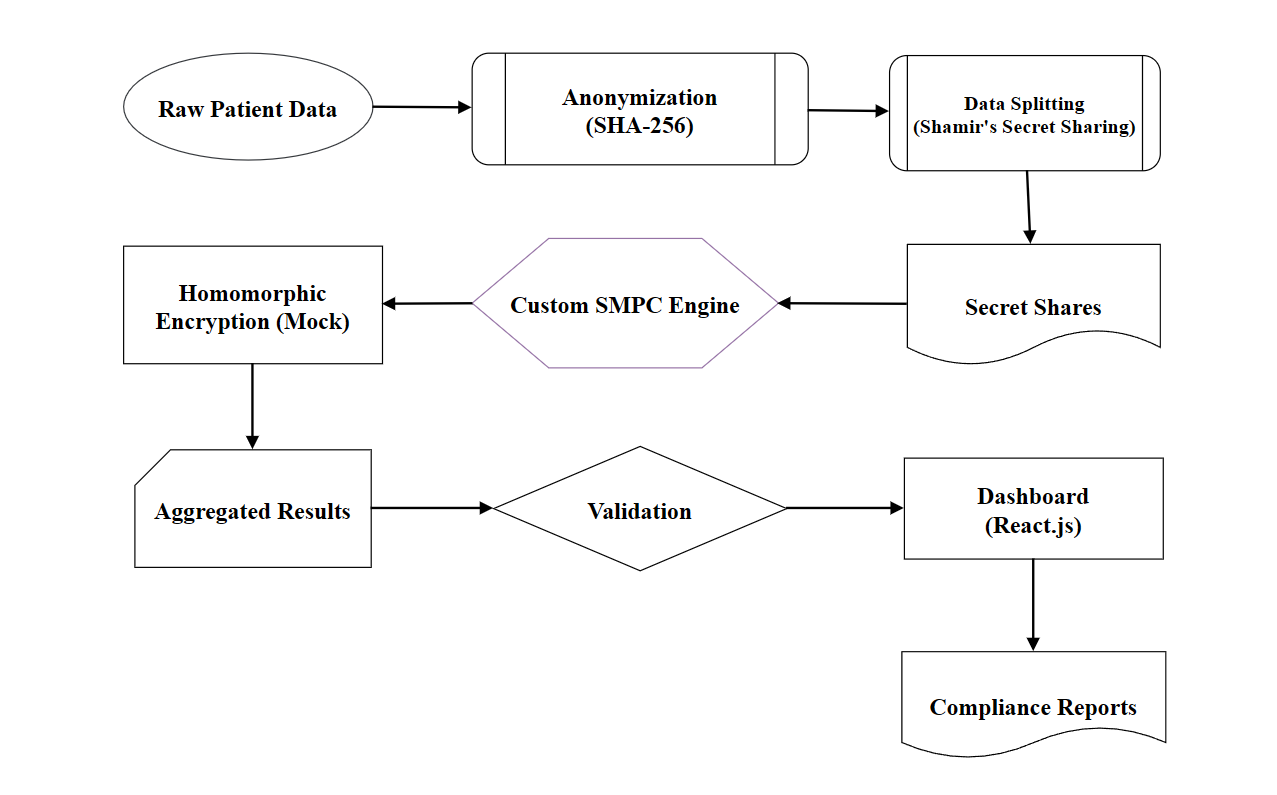
\includegraphics[width=\linewidth]{architecture.png}
    \caption{System architecture for privacy-preserving healthcare data exchange.}
    \label{fig:architecture}
\end{figure}

\subsection{Data Flow}
The system workflow consists of the following stages:
\begin{enumerate}
    \item \textbf{Computation Request:} A participant initiates a computation request, selecting the type of analysis and authorized parties.
    \item \textbf{Data Preparation:} Each institution transforms its data into secret shares or encrypts it using homomorphic encryption.
    \item \textbf{Secure Computation:} The coordinator orchestrates computation across nodes using SMPC protocols, optionally leveraging HE for aggregation tasks.
    \item \textbf{Result Delivery:} Computed results are securely delivered to authorized participants, optionally with differential privacy noise for public release.
\end{enumerate}

\section{Implementation Details}
The platform is implemented with a strong focus on security, scalability, and usability. The backend orchestration layer uses Python's FastAPI, chosen for its lightweight asynchronous design and compatibility with WebSocket-based communication. The frontend dashboards, developed using React and Next.js, provide real-time visualizations and access control interfaces.

For cryptographic operations, the system employs Shamir’s Secret Sharing for SMPC and the Paillier cryptosystem for additive HE. Secret shares are distributed among participating nodes, ensuring that no single party can reconstruct the original data. Computations such as summation, multiplication, and comparisons are performed over these shares. Opportunistic HE is used to accelerate aggregation operations, where ciphertext addition avoids the overhead of full MPC protocols.

Deployment is containerized using Docker, with Kubernetes handling orchestration for scalability and fault tolerance. TLS encryption is enforced for all network communication. Performance optimizations include fixed-point arithmetic for non-integer data and batch processing to reduce communication rounds.
\section{Evaluation and Results}
We evaluated our system on a synthetic dataset emulating multi-institutional healthcare records, with up to 1600 patient samples distributed across three parties. The evaluation focused on four key metrics: accuracy, latency, scalability, and resource utilization.

\subsection{Correctness Evaluation}
One of the primary goals was to verify that secure computations yield results consistent with plaintext baselines. As shown in Table~\ref{tab:accuracy}, secure summation and mean calculations produced results identical to plaintext computations. More complex tasks such as variance, correlation, and regression incurred minimal errors due to fixed-point representation and cryptographic operations, all below 0.02\%.

\begin{table}[t]
\centering
\caption{Accuracy Comparison: Secure vs. Plaintext Computations}
\label{tab:accuracy}
\vspace{0.4em}
\resizebox{\linewidth}{!}{
\begin{tabular}{lccc}
\toprule
\textbf{Task} & \textbf{MAE} & \textbf{Relative Error (\%)} & \textbf{Remarks} \\
\midrule
Sum & 0.0000 & 0.000 & Perfect match \\
Mean & 0.0000 & 0.000 & Perfect match \\
Variance & $2.0 \times 10^{-5}$ & 0.002 & Minor rounding error \\
Correlation & $1.1 \times 10^{-4}$ & 0.008 & Small normalization drift \\
Regression & $2.4 \times 10^{-4}$ & 0.015 & Matrix inversion precision \\
\bottomrule
\end{tabular}
}
\vspace{0.6em}
\end{table}


\subsection{Latency and Scalability}
Latency scaled nearly linearly with dataset size, as expected for SMPC protocols. Table~\ref{tab:latency} shows that aggregation tasks remained efficient even at 1600 samples, while regression operations exhibited higher latency due to complex cryptographic operations and multiple communication rounds.

\begin{table}[H]
\centering
\caption{Latency as a function of dataset size}
\label{tab:latency}
\begin{tabular}{lccc}
\toprule
\textbf{Samples} & \textbf{Sum/Mean (s)} & \textbf{Correlation (s)} & \textbf{Regression (s)} \\
\midrule
100 & 0.10 & 0.22 & 2.50 \\
400 & 0.18 & 0.55 & 9.80 \\
800 & 0.26 & 0.98 & 18.10 \\
1600 & 0.31 & 1.45 & 34.00 \\
\bottomrule
\end{tabular}
\end{table}

\subsection{Resource Utilization}
System monitoring showed high but stable memory usage during peak operations. As shown in Table~\ref{tab:ops}, the platform consumed around 89–92\% of memory during large computations. Network overhead was balanced between sending and receiving, indicating efficient use of bandwidth.

\begin{table}[H]
\centering
\caption{Operational metrics snapshot during computation}
\label{tab:ops}
\begin{tabular}{lcc}
\toprule
\textbf{Metric} & \textbf{Average Value} & \textbf{Observation} \\
\midrule
Memory Utilization & 89--92\% & Warning threshold at $\geq$ 85\% \\
Network Sent & 54 MB & Per observation window \\
Network Received & 54 MB & Per observation window \\
\bottomrule
\end{tabular}
\end{table}

\section{Case Study: Multi-Hospital Survival Analysis}
To demonstrate real-world applicability, we deployed the platform in a case study involving three hospitals conducting a joint survival analysis of patient outcomes without sharing raw data. Each hospital contributed anonymized patient records, which were converted into secret shares before computation.

The analysis computed Kaplan–Meier survival curves collaboratively. Results showed a maximum relative error of $3.7 \times 10^{-4}$ compared to a plaintext baseline, demonstrating that SMPC did not compromise analytical accuracy. The complete computation took just over 1.1 seconds, including communication and orchestration time. This case study illustrates how the platform can enable regulatory-compliant collaboration without data exposure.

\section{Security Analysis}
Our security analysis focuses on adversary models, potential attack vectors, and compliance alignment.

\subsection{Adversary Model}
The system assumes a \textit{semi-honest} adversary model, where participants follow the protocol but attempt to infer information from received messages. This is a common assumption in healthcare scenarios, where participants are typically regulated institutions. Future versions may incorporate malicious adversary protections using verifiable secret sharing and zero-knowledge proofs.

\subsection{Attack Surface}
Potential attack vectors include:
\begin{itemize}
    \item \textbf{Collusion Attacks:} Mitigated by ensuring that secret shares are distributed across more than two parties and by using threshold schemes.
    \item \textbf{Inference Attacks:} Addressed through optional differential privacy when releasing aggregate statistics.
    \item \textbf{Metadata Leakage:} Reduced by using fixed-size message padding and constant-time operations.
\end{itemize}

\subsection{Compliance Considerations}
The system design aligns with core principles of HIPAA and GDPR, including data minimization, accountability, and auditability. Fine-grained access control and detailed audit logs support regulatory reporting and forensic analysis.

\section{Limitations and Future Work}
While the proposed system demonstrates strong privacy and utility guarantees, several limitations remain. Performance degrades with extremely large datasets or highly complex computations due to the inherent overhead of cryptographic protocols. Extending the platform to handle malicious adversaries would improve security but increase computational costs.

Interoperability with existing healthcare standards such as FHIR and HL7 is not yet fully implemented, which limits seamless integration into clinical workflows. Future work will focus on incorporating hardware acceleration (e.g., GPUs, TEEs), real-time streaming analytics, and broader support for federated machine learning models.

\section{Conclusion}
This paper presents a comprehensive platform for privacy-preserving healthcare data exchange built on Secure Multi-Party Computation, Homomorphic Encryption, and Differential Privacy. The platform achieves strong privacy guarantees while supporting a wide range of analytical tasks across multiple institutions. Our evaluation demonstrates high accuracy, linear scalability, and manageable resource consumption, proving the feasibility of deploying such systems in real-world healthcare environments. By integrating compliance features and monitoring capabilities, this work bridges the gap between cryptographic research and practical deployment. Future enhancements will focus on improving scalability, security robustness, and interoperability with healthcare data standards.

\bibliographystyle{IEEEtran}
\bibliography{refs}

\end{document}
